%===================================== CHAPTER 5 Requirements specification =================================

\chapter{Requirements specification}

This chapter describe the requirements for the application. The chapter is divided into two sections: one section describing the functional requirements, another that describes the non-functional requirements.

\section{Functional requirements}

The requirements document for this project can be found in appendix A. This document contains a description of the functional requirements. The requirements were elicited and agreed upon with the customer in meetings and formalized in the requirements document. In early customer meetings the functionalities of the application were discussed informally. The group wrote a requirements document which was discussed at subsequent meetings. In these meetings each proposed requirement was refined and given a priority. The priorities were assigned using a high-medium-low scale. This priority has guided the sequence of progress in the project. In addition, the group elicited its own prioritization where all the requirements were ranked, each with its own unique number ranging from 1 to the total number of requirements. The description of requirements in this chapter is less formal and more high-level than the one found in the requirements document. 

\subsection{Summary of the functional requirements}
\label{subsec:summary_functional_requirements}

This section provides an informal summary of the main requirements that were initially proposed. These requirements have been detailed and refined in the use case section, as well as the functional requirements document. \newline

Sign up/Sign in view: The application should in some way be able to identify users, but keep them as anonymous as possible. For research purposes, personal data like age group and gender should be collected.\newline

Preferences/Settings: The user should be able to specify some preferences regarding cultural categories and the use of location from the device.\newline

Main view: Browse recommended stories: The application should provide the user with recommended stories based on the user’s preferences. The user is provided with three choices on each story: to read it now, to reject it or to save it for later.\newline

Story view: The application should present a chosen story in an clear way that respect the work of the author and resemble the presentation on the Digitalt fortalt website. Every story should also include a link to the corresponding story on Digitalt fortalt. The user should be given the opportunity to rate the story and to tag the story. In addition, the application should provide an explanation of why the story was recommended.\newline

Collected story view: The application should keep a collection of stories that the user have been recommended and that have not been rejected. The user should be able to filter this list based on the status of the story (to-read, read, reviewed) or tags (predefined tags like “Favorites” or the user's own tags).\newline

Notifications: The application should provide the user with the opportunity to set a preferred time it wants to receive a notification about a new recommended story on their device. At the set time, the application should send the notification. In addition, the application should notify the user when a story is missing a rating.\newline

About / help site: The application should include an about site, which explains the context in which the application was created. \newline

Personalization: When recommending stories the application should employ both content-based filtering and collaborative filtering algorithms.\newline

Research: The application should gather information about the use. This data is to be presented to the customer at SINTEF through a simple interface.\newline

\subsection{Use cases}
\label{subsec:use_cases}

The use cases in this section give an overview of the interaction with the system. In the requirements document one can find references to the use cases for requirements that involve external interaction.\newline

A use case is a simple scenario that identifies actors involved in an interaction with a system and describe this interaction[AS1]. Actors are entities outside the system interacting with it to accomplish some task. This can be a human using the system or it can be some other system. In eliciting requirements in a software development process, use cases are particularly effective in making it clear what is expected of the system in terms of user interaction. A use case diagram is usually presented with ellipses and stick figures. The ellipses represent the use case and the stick figures represent the actors (even if the actor is an external system). This simple notation is often complemented by a textual description which provide more detail.\newline

The use cases in this section define interactions between an actor and the application. Actors in these use cases are the user of the system, the device on which the application run, and Digitalt fortalt . The use cases consist of a textual description accompanied by a visual representation in the form of use case diagrams. The textual description follows a template which consists of these items:
\begin{itemize}
\item ID: A unique identification for the use case.
\item Name: A short text describing the goal of the use case.
\item Brief description: This is a more elaborate explanation of the use case than the above.
\item Actors: These are the users/systems outside the application interacting with it.
\item Priority: A metric describing the priority of this use case. This metric is derived from the functional requirements document, and uses a high-medium-low scale.
\item Preconditions: Describe what state the system should be in before the use case can start. Typically, some of the other use cases are already performed to set up the use case.
\item Basic flow: This describe the normal flow from preconditions to postconditions in a numbered list.
\item Alternate flow: A description of scenarios that differ from the basic flow described above. This includes exceptions and errors. It is also presented as a list, but the numbering in this list refers to the items in the basic flow list. The items in this list do not relate to each other.
\item Postconditions: Describe what state the system should be in after the use case is performed.
\end{itemize}

\begin{table}[htp]
	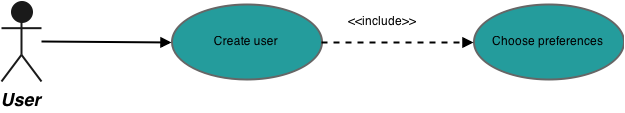
\includegraphics[width=\textwidth]{fig/U1}
	\centering
	\caption{U1. Create profile}
	\begin{tabular}[b]{|l | l|}\hline
		\textbf{ID} 				& U1									\\\hline
		\textbf{Name} 				& Create recoverable profile.			\\\hline
		\textbf{Brief description}	& Enter mail to register. 				\\\hline
		\textbf{Actors} 			& User									\\\hline
		\textbf{Priority}			& High									\\\hline
		\textbf{Preconditions}		& Application installed					\\\hline&\\[-2ex]
		\textbf{Basic flow}			& \begin{minipage}{5in}
									  \begin{enumerate}[noitemsep]
										\item User clicks on register new user
										\item User fills in mail into a registration form
										\item Input validated
										\item User finishes the registration and the syestem saves the user ID
									  \end{enumerate}						
									  \end{minipage}						\\\hline&\\[-2ex]
		\textbf{Alternate flow}		& \begin{minipage}{5in}
									  \begin{enumerate}[noitemsep]
										\item User skips registration and starts using the system
										\item The system stores the new user by an ID internally
									  \end{enumerate}
									 \end{minipage}							\\\hline
		\textbf{Postconditions}		& User is created and saved by the system\\\hline
	\end{tabular}
\end{table}

\begin{table}[htp]
	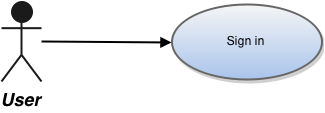
\includegraphics[width=0.5\textwidth]{fig/U2}
	\centering
	\caption{U2. Sign in}
	\begin{tabular}[b]{|l | l|}\hline
		\textbf{ID} 				& U2									\\\hline
		\textbf{Name} 				& Sign in.								\\\hline
		\textbf{Brief description}	& Enter email address to sign in. 		\\\hline
		\textbf{Actors} 			& User									\\\hline
		\textbf{Priority}			& High									\\\hline
		\textbf{Preconditions}		& User has already registered			\\\hline&\\[-2ex]
		\textbf{Basic flow}			& \begin{minipage}{5in}
			\begin{enumerate}[noitemsep]
				\item User clicks on sign in
				\item User fills in mail into form
				\item System checks email address. User id returned
				\item Main view displayed
			\end{enumerate}						
		\end{minipage}						\\\hline&\\[-2ex]
		\textbf{Alternate flow}		& \begin{minipage}{5in}
			\begin{enumerate}[noitemsep]
				\item User not found
				\item Error message displayed, go to 2.
			\end{enumerate}
		\end{minipage}							\\\hline
		\textbf{Postconditions}		& User is logged in to the system\\\hline
	\end{tabular}
\end{table}

\begin{table}[htp]
	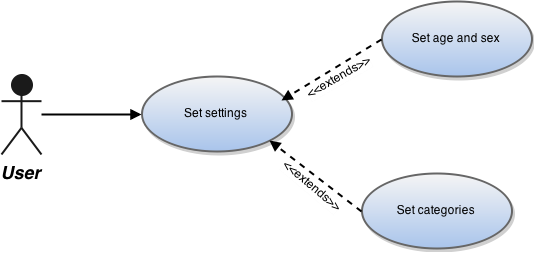
\includegraphics[width=\textwidth]{fig/U3}
	\centering
	\caption{U3. Set initial settings}
	\begin{tabular}[b]{|l | p{13cm}|}\hline
		\textbf{ID} 				& U3									\\\hline
		\textbf{Name} 				& Set initial settings.					\\\hline
		\textbf{Brief description}	& Specify user information to be used for receiving stories. \\\hline
		\textbf{Actors} 			& User									\\\hline
		\textbf{Priority}			& High									\\\hline
		\textbf{Preconditions}		& Application installed					\\\hline&\\[-2ex]
		\textbf{Basic flow}			& \begin{minipage}{5in}
			\begin{enumerate}[noitemsep]
				\item User is initially asked to fill a form about preferences by the system
					\begin{enumerate}
						\item Personal info: age group and sex
						\item Cultural category preferences
					\end{enumerate}
				\item The system saves information about the user’s preferences
			\end{enumerate}						
		\end{minipage}						\\\hline&\\[-2ex]
		\textbf{Alternate flow}		& \begin{minipage}{5in}
			\begin{enumerate}[noitemsep]
				\item User clicks on settings in order to change preferences
			\end{enumerate}
		\end{minipage}							\\\hline
		\textbf{Postconditions}		& The system has information about the user in order to provide personalized story recommendations.\\\hline
	\end{tabular}
\end{table}

\begin{table}[htp]
	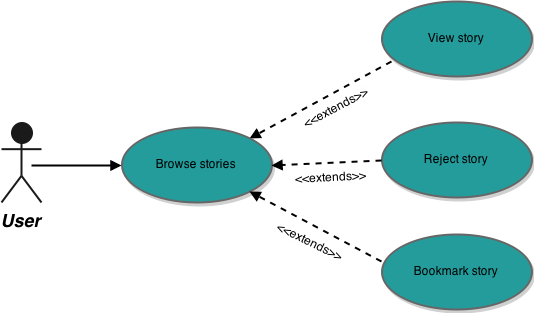
\includegraphics[width=\textwidth]{fig/U4}
	\centering
	\caption{U4. Browse recommended stories}
	\begin{tabular}[b]{|l | l|}\hline
		\textbf{ID} 				& U4									\\\hline
		\textbf{Name} 				& Browse recommended stories.			\\\hline
		\textbf{Brief description}	& User is shown a list of recommended stories to choose from. 		\\\hline
		\textbf{Actors} 			& User									\\\hline
		\textbf{Priority}			& High									\\\hline
		\textbf{Preconditions}		& Preferences already set				\\\hline&\\[-2ex]
		\textbf{Basic flow}			& \begin{minipage}{5in}
			\begin{enumerate}[noitemsep]
				\item User is shown a list of recommended stories
				\item User does one of the three following actions on a story:
					\begin{enumerate}
						\item Choose to read the story now
						\item Reject the story
						\item Add story to list  
					\end{enumerate}
				\item If option (b) or (c) is chosen the user is shown a recommendation list without the story
			\end{enumerate}						
		\end{minipage}						\\\hline&\\[-2ex]
		\textbf{Alternate flow}		& \begin{minipage}{5in}
			\begin{enumerate}[noitemsep]
				\item If the user chose to read the story now, the story - and not the updated recommendation list - will be shown.
			\end{enumerate}
		\end{minipage}							\\\hline
		\textbf{Postconditions}		& The system has stored information about the choice of the user.\\\hline
	\end{tabular}
\end{table}

\begin{table}[htp]
	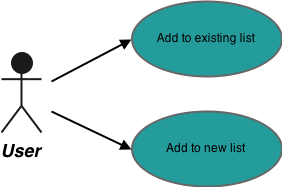
\includegraphics[width=0.5\textwidth]{fig/U5}
	\centering
	\caption{U5. Add story to list}
	\begin{tabular}[b]{|l | l|}\hline
		\textbf{ID} 				& U5									\\\hline
		\textbf{Name} 				& Add story to list.					\\\hline
		\textbf{Brief description}	& Put a story in to-read list or user-defined  list. 		\\\hline
		\textbf{Actors} 			& User									\\\hline
		\textbf{Priority}			& Medium								\\\hline
		\textbf{Preconditions}		& User is registered and signed in		\\\hline&\\[-2ex]
		\textbf{Basic flow}			& \begin{minipage}{5in}
			\begin{enumerate}[noitemsep]
				\item User opens a story to read
				\item User clicks the bookmark button in the story and selects the desired collections to put the story in.
				\item Story will be put in the selected list
			\end{enumerate}						
		\end{minipage}						\\\hline&\\[-2ex]
		\textbf{Alternate flow}		& \begin{minipage}{5in}
			\begin{enumerate}[noitemsep]
				\item The desired collection does not exist. The user clicks to add new collection.
			\end{enumerate}
		\end{minipage}							\\\hline
		\textbf{Postconditions}		& Story will be added to and/or removed from various lists according to user's actions\\\hline
	\end{tabular}
\end{table}

\begin{table}[htp]
	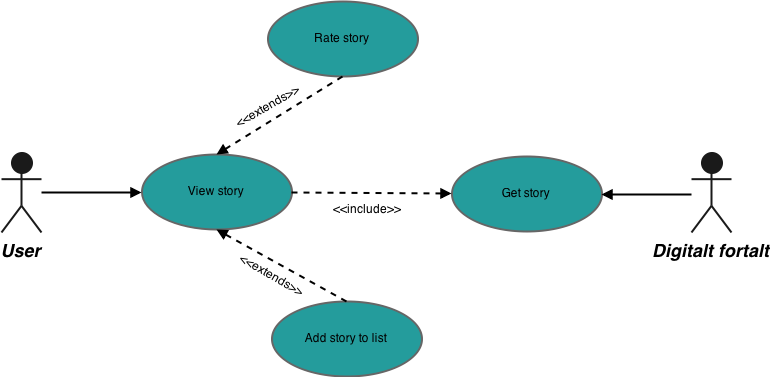
\includegraphics[width=\textwidth]{fig/U6}
	\centering
	\caption{U6. View story}
	\begin{tabular}[b]{|l | l|}\hline
		\textbf{ID} 				& U6									\\\hline
		\textbf{Name} 				& View story.							\\\hline
		\textbf{Brief description}	& Display media (text, images, video, sound clips) related to the story selected. 		\\\hline
		\textbf{Actors} 			& User, Digitalt fortalt				\\\hline
		\textbf{Priority}			& High									\\\hline
		\textbf{Preconditions}		& The story is in the list of recommended stories or favorites			\\\hline&\\[-2ex]
		\textbf{Basic flow}			& \begin{minipage}{5in}
			\begin{enumerate}[noitemsep]
				\item User selects story
				\item Display:
					\begin{enumerate}
						\item Available media files
						\item Link to story on Digitalt fortalt
						\item Explanation of why the story was recommended
					\end{enumerate}
				\item User selects media type (text default)
			\end{enumerate}						
		\end{minipage}						\\\hline&\\[-2ex]
		\textbf{Alternate flow}		& \begin{minipage}{5in}
		\end{minipage}							\\\hline
		\textbf{Postconditions}		& The story is shown according to the user preferences\\\hline
	\end{tabular}
\end{table}

\begin{table}[htp]
	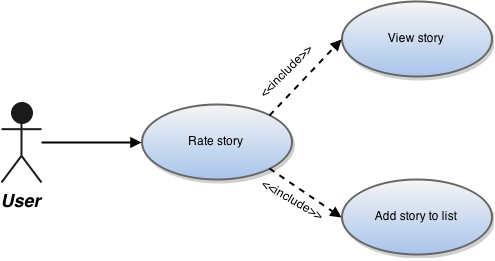
\includegraphics[width=\textwidth]{fig/U7}
	\centering
	\caption{U7. Rate story}
	\begin{tabular}[b]{|l | l|}\hline
		\textbf{ID} 				& U7									\\\hline
		\textbf{Name} 				& Give feedback / rating.				\\\hline
		\textbf{Brief description}	& Give a rating on a story. 			\\\hline
		\textbf{Actors} 			& User									\\\hline
		\textbf{Priority}			& High									\\\hline
		\textbf{Preconditions}		& User has opened a story for reading	\\\hline&\\[-2ex]
		\textbf{Basic flow}			& \begin{minipage}{5in}
			\begin{enumerate}[noitemsep]
				\item After reading the story,  the user clicks on a rating to give feedback on the story
				\item The system saves the rating
				\item Story will be put in read list
			\end{enumerate}						
		\end{minipage}						\\\hline&\\[-2ex]
		\textbf{Alternate flow}		& \begin{minipage}{5in}
			\begin{enumerate}[noitemsep]
				\item User does not give a rating on the story before closing it
				\item The system reminds the user to rate the story at a later time
			\end{enumerate}
		\end{minipage}							\\\hline
		\textbf{Postconditions}		& The rating of the story from the user is saved\\\hline
	\end{tabular}
\end{table}

\begin{table}[htp]
	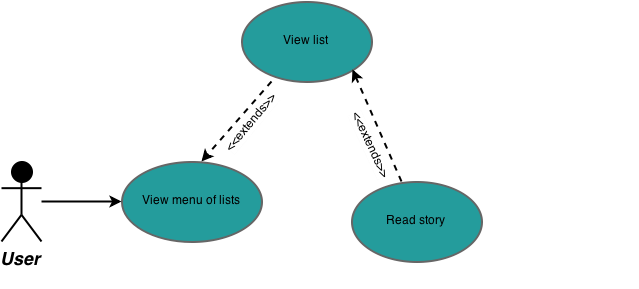
\includegraphics[width=\textwidth]{fig/U8}
	\centering
	\caption{U8. View list}
	\begin{tabular}[b]{|l | l|}\hline
		\textbf{ID} 				& U8									\\\hline
		\textbf{Name} 				& View list.							\\\hline
		\textbf{Brief description}	& View list of collected stories (favorites,to-read,tags defined by user). 			\\\hline
		\textbf{Actors} 			& User									\\\hline
		\textbf{Priority}			& Medium								\\\hline
		\textbf{Preconditions}		& User is registered and signed in		\\\hline&\\[-2ex]
		\textbf{Basic flow}			& \begin{minipage}{5in}
			\begin{enumerate}[noitemsep]
				\item User selects list from menu
				\item List of stories shown
			\end{enumerate}						
		\end{minipage}						\\\hline&\\[-2ex]
		\textbf{Alternate flow}		& \begin{minipage}{5in}
			\begin{enumerate}[noitemsep]
				\item No stories found
				\item Display message “No stories found”
			\end{enumerate}
		\end{minipage}							\\\hline
		\textbf{Postconditions}		& User is shown all of the stories collected\\\hline
	\end{tabular}
\end{table}

\begin{table}[htp]
	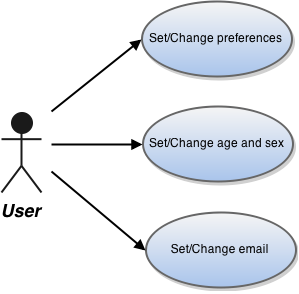
\includegraphics[width=0.5\textwidth]{fig/U9}
	\centering
	\caption{U9. Specify settings}
	\begin{tabular}[b]{|l | l|}\hline
		\textbf{ID} 				& U9									\\\hline
		\textbf{Name} 				& Specify settings.						\\\hline
		\textbf{Brief description}	& Specify and change system settings. 	\\\hline
		\textbf{Actors} 			& User									\\\hline
		\textbf{Priority}			& High									\\\hline
		\textbf{Preconditions}		& User is signed in						\\\hline&\\[-2ex]
		\textbf{Basic flow}			& \begin{minipage}{5in}
			\begin{enumerate}[noitemsep]
				\item While logged in, user clicks on settings
				\item User edits the data in settings
					\begin{enumerate}
						\item Category preferences
						\item Age group / sex
						\item User e-mail
					\end{enumerate}
				\item The system saves the new settings
			\end{enumerate}						
		\end{minipage}						\\\hline&\\[-2ex]
		\textbf{Alternate flow}		& \begin{minipage}{5in}
		\end{minipage}							\\\hline
		\textbf{Postconditions}		& Settings are changed and saved\\\hline
	\end{tabular}
\end{table}

\begin{table}[htp]
	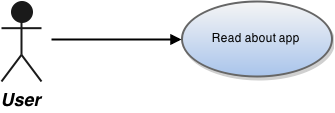
\includegraphics[width=0.5\textwidth]{fig/U10}
	\centering
	\caption{U10. Read about app}
	\begin{tabular}[b]{|l | l|}\hline
		\textbf{ID} 				& U10									\\\hline
		\textbf{Name} 				& Read about app.						\\\hline
		\textbf{Brief description}	& Basic info about the application. 	\\\hline
		\textbf{Actors} 			& User									\\\hline
		\textbf{Priority}			& High									\\\hline
		\textbf{Preconditions}		& User is signed in						\\\hline&\\[-2ex]
		\textbf{Basic flow}			& \begin{minipage}{5in}
			\begin{enumerate}[noitemsep]
				\item While logged in, user clicks on settings
				\item User clicks on read about app and is presented with information about the app
			\end{enumerate}						
		\end{minipage}						\\\hline&\\[-2ex]
		\textbf{Alternate flow}		& \begin{minipage}{5in}
		\end{minipage}							\\\hline
		\textbf{Postconditions}		& \\\hline
	\end{tabular}
\end{table}

\section{Non-functional requirements}
\label{sec:non-functional_requirements}

A general requirement for the project was to use english as language in all parts related to the documentation of the application, while the language in the application would be norwegian. Other general requirements concerned the platforms the application should run on. It was decided that it should run on both Android and iOS, and that the design of the application should approach a native feel as much as possible on these platforms.\newline

To make better decisions at a top-level design perspective, and to make better decisions on a component and implementation level, the team wanted the customer to rank each of the quality attributes below. The basis for the list and its descriptions are sourced in Software Architecture in Practice (REF). The ranked list was helpful in choosing the solutions that were most inline with the customer’s needs. Normally there would be a system for measuring and quantifying each of the attributes, but this would broaden the scope and workload of the project and instead this was used as a prioritized list assisting the development, since this was believed by the team to be adequate in terms of the scope and length of the project.\newline

There are many more quality attributes but this list describes the most generic ones, plus some specific attributes that the team believed might suit the project. Also, keep in mind that there are a lot of crossover attributes(e.g.. Maintainability/Testability may increase availability)\newline
\begin{itemize}
\item Availability: How important is the reliability of the product. The easy representation to think of this is uptime of the service.
\item Interoperability: How important is the ability for the system to work together with other systems. (e.g. making use of specific communication protocols or the use of a specified data format)
\item Modifiability: How important and how easy should the product be able to be changed after it is finalized? (e.g. making changes to the UI)
\item Performance: How important is time and speed of the system? (e.g. response time for retrieving stories)
\item Security: How important is the system’s ability to protect data and information from unauthorized access? (e.g. losing personalized data)
\item Testability: How important is the ability to set up tests for the system (e.g. setting up automated test for components and parts of the system)
\item Usability: How easy is it for the user to accomplish a desired task, and what kind of user support should the system focus on. (e.g. tutorials or hints)
\item Monitorability: How important is the ability to monitor how the system while its executing. (e.g. statistics etc.)
\item Other: These have been considered not very relevant for the project due to various reasons; variability, portability, development distributability, scalability, deployability, mobility, safety, marketability
\end{itemize}

(TODO Supplement: diagram non-functional requirement)

\cleardoublepage

